Per la pianificazione, sono stati individuati 5 periodi, scelti in base ai processi primari coinvolti. Ogni periodo contiene diverse attività. Nella pianificazione, verrà impiegata tale numerazione:
\begin{center}
	[\textbf{Periodo}].[\textbf{Attività}]
\end{center}
se non le attività non vengono raggruppate,
\begin{center}
	[\textbf{Periodo}].[\textbf{Insieme di attività}].[\textbf{Attività}]
\end{center}
altrimenti.\\
La numerazione, sia per i periodi sia per gli insieme di attività sia per le singole attività, è sequenziale.

\subsection{Periodo di Avvio e di Analisi}
	\subsubsection{Periodo di Avvio (2018-12-4 - 2018-12-17)}
		Nel periodo di avvio hanno luogo le seguenti attività:
		\begin{enumerate}[label = 1.\arabic*)]
			\item ricerca degli strumenti (2018-12-4 - 2018-12-14): tutti i membri del gruppo effettuano le ricerche sui possibili strumenti utili alle attività di avvio e di analisi dei requisiti;
			\item prima normazione (2018-12-5 - 2018-12-14): gli amministratori redigono le norme di progetto concordate per i processi di supporto e organizzativi;
			\item studio di fattibilità (2018-12-4 - 2018-12-8): gli analisti effettuano lo studio di fattibilità dei capitolati;
			\item pianificazione di progetto (2018-12-7 - 2018-12-13): il responsabile redige il piano di progetto, riportando modello di sviluppo, analisi dei rischi e la pianificazione per le prime attività dell'analisi dei requisiti;
			\item verifica dei documenti (2018-12-15 - 2018-12-16): i verificatori controllano se i documenti siano corretti.
		\end{enumerate}
		
	\subsubsection{Periodo di Analisi (2018-12-17 - 2018-01-21)}	
		\paragraph{Pianificazione (2018-12-17 - 2018-12-23)\\} Il periodo di analisi dei requisiti inizia con le attività di:
			\begin{enumerate}[label = 2.1.\arabic*)]
				\item pianificazione di progetto (2018-12-17 - 2018-12-21): il responsabile effettua il resoconto del periodo di avvio e pianifica in maniera più dettagliata le attività di analisi dei requisiti; 
				\item pianificazione della qualifica (2018-12-17 - 2018-12-21): i verificatori redigono il resoconto del periodo di avvio e gli amministratori effettuano i primi incrementi per il piano di qualifica;
				\item normazione (2018-12-17 - 2018-12-21): gli amministratori redigono in maniera precisa e completa le norme per l'attività di analisi;
				\item verifica dei piani e delle norme (2018-12-21 - 2018-12-23).
			\end{enumerate}
		
		\paragraph{Analisi dei requisiti (2018-12-19 - 2018-02-09)\\} La parte centrale del periodo di analisi dei requisiti è costituita dalle attività di:
			\begin{enumerate}[label = 2.2.\arabic*)]
				\item analisi dei requisiti del sistema (2018-12-19 - 2018-12-27): gli analisti svolgono la prima analisi dei requisiti del sistema;
				\item incrementi al Piano di Qualifica (2018-12-26 - 2018-12-30): gli analisti introducono nel piano i test di sistema in base a quanto scaturito dall'analisi dei requisiti;
				\item verifica dell'analisi dei requisiti di sistema (2018-12-29 - 2018-12-31)
				\item verifica del Piano di Qualifica (2018-01-09 - 2019-01-03)
				\item incrementi all'analisi dei requisiti (2019-01-02 - 2019-01-08): gli analisti aggiungono degli incrementi all'analisi di sistema
				\item verifica degli incrementi all'analisi dei requisiti (2019-01-09 - 2019-01-11)
				\item incrementi al Piano di Progetto (2019-01-07 - 2019-01-10): il responsabile redige la parte di rendicontazione e consuntivo del piano di progetto da presentare alla Revisione dei Requisiti.
				\item incrementi al Piano di Qualifica (2019-01-07 - 2019-01-10): i verificatori redigono la parte di rendicontazione del piano di qualifica da presentare alla Revisione dei Requisiti, aggiungendo i risultati delle misurazioni effettuate, e gli analisti aggiungono i restanti test di sistema.
				\item verifica dei piani di Progetto e Qualifica (2019-01-11 - 2019-01-12)
				\item preparazione alla presentazione (2019-01-15 - 2019-01-20);
				\item analisi dei requisiti software (2019-02-01 - 2019-02-05): gli analisti effettuano l'analisi dei requisiti software. Quest'attività è successiva al primo incremento di progettazione architetturale.
				\item verifica dell'analisi dei requisiti (2019-02-07 - 2019-02-09)				
			\end{enumerate}

	\newpage
	\begin{figure}[!hbtp]
		\centering
		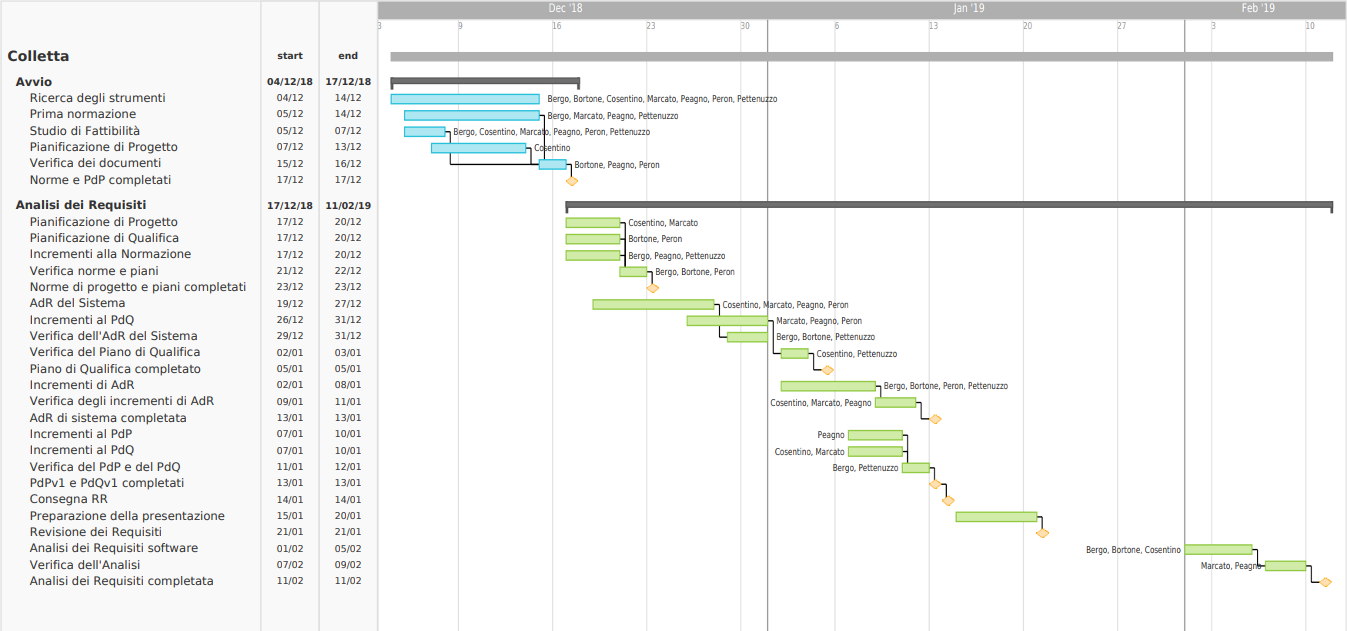
\includegraphics[scale=0.5,angle=90]{images/ganttan.png}
		\caption{Diagramma di Gantt per il periodo di avvio e di analisi}
	\end{figure}
	
	\newpage
	\subsection{Progettazione}	
	
	\newpage
	\subsection{Realizzazione (2019-02-21 - 2019-05-01)}
		\begin{enumerate}[label= 4.\arabic*)]
			\item incrementi alla normazione (2019-02-21 - 2019-02-24): gli amministratori redigono le norme per il processo di realizzazione;
			\item incrementi al Piano di Progetto (2019-02-21 - 2019-02-24): il responsabile pianifica gli incrementi di codifica e la realizzazione del prodotto;
			\item incrementi al Piano di Qualifica (2019-02-21 - 2019-02-24): i progettisti indicano i test di unità per i moduli da realizzare durante la codifica;
			\item verifica dei piani e delle norme (2019-02-25 - 2019-02-26);
			\item codifica (2019-02-24 - 2019-03-02): i programmatori realizzano i moduli indicati dai progettisti secondo l'ordine stabilito
			\item verifica (2019-03-04 - 2019-03-05): verifica del codice prodotto durante la codifica
			\item incrementi di codifica (2019-03-17 - 2019-03-23)
			\item verifica degli incrementi (2019-03-24 - 2019-03-25)
			\item incrementi di codifica (2019-03-29 - 2019-04-04)
			\item verifica degli incrementi (2019-04-05 - 2019-04-07)
			\item produzione del manuale (2019-03-30 - 2019-04-05): i progettisti si occupano di scrivere il manuale utente e il manuale dello sviluppatore;
			\item verifica del manuale (2019-04-06 - 2019-04-08);
			\item incrementi al Piano di Progetto (2019-04-06 - 2019-04-09): il responsabile redige la parte di rendicontazione e consuntivo del piano di progetto da presentare alla Revisione di Qualifica;
			\item incrementi al Piano di Qualifica (2019-04-06 - 2019-04-09): i verificatori redigono la parte di rendicontazione del piano di qualifica da presentare alla Revisione di Qualifica, aggiungendo i risultati delle misurazioni effettuate;
			\item verifica dei piani di Qualifica e di Progetto (2019-04-10 - 2019-04-11);
			\item preparazione della presentazione (2019-04-13 - 2019-04-18);
			\item incrementi di codifica (2019-04-26 - 2019-04-29): i programmatori effettuano gli incrementi di codifica basati sulle correzioni effettuate dall'ultimo incremento di progettazione di dettaglio.
			\item verifica degli incrementi (2019-04-30 - 2019-05-1).
		\end{enumerate}
		
	\newpage
	\begin{figure}[!hbtp]
		\centering
		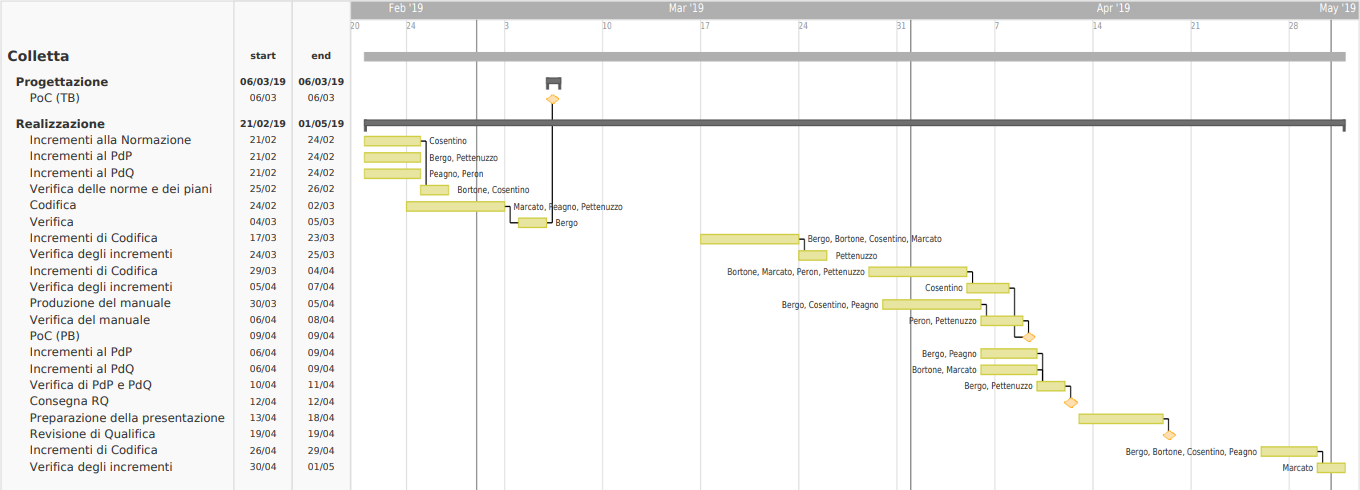
\includegraphics[scale=0.5, angle=90]{images/ganttreal.png}
		\caption{Diagramma di Gantt per il periodo di realizzazione}
	\end{figure}
	
	\newpage
	\subsection{Validazione}
		